
% Add "answers" option to print the answers
\documentclass[addpoints,answers]{exam}
%\documentclass[addpoints]{exam}

\usepackage[utf8]{inputenc}
\usepackage{calc}
\usepackage{listings}
\usepackage{xcolor}
\usepackage{xspace}

\definecolor{codegreen}{rgb}{0,0.6,0}
\definecolor{codegray}{rgb}{0.5,0.5,0.5}
\definecolor{codepurple}{rgb}{0.58,0,0.82}

\lstdefinestyle{Cstyle}{
    commentstyle=\color{codegreen},
    keywordstyle=\color{magenta},
    numberstyle=\tiny\color{codegray},
    stringstyle=\color{codepurple},
    basicstyle=\ttfamily\small,
    breakatwhitespace=true,         
    breaklines=true,                 
    captionpos=b,                    
    keepspaces=true,                 
    numbers=left,                    
    numbersep=5pt,                  
    showspaces=false,                
    showstringspaces=false,
    showtabs=false,                  
    tabsize=4
}

\lstset{style=Cstyle}

% \makebox[\textwidth]{Name:\enspace\hrulefill}
%  
% \vspace{5mm}
%\makebox[\textwidth]{Instructor’s name:\enspace\hrulefill}

\newcommand{\truefalse}
{		\begin{checkboxes}
			 \choice True
			 \choice False. Explanation: 
		\end{checkboxes}
		\vspace{10pt}
}

\newcommand{\answerspace}[1]
{
	\ifprintanswers
	\else
		\setlength{\mylength}{10pt}%
		%\noindent\rule{\mylength}{20pt}
		%\vspace{\fpeval{1.2*(#1)}}
		\vspace{#1\mylength}
	\fi
}
\newlength{\mylength}

\newcommand\pf[1]{\textcolor{red}{PF: #1}}
\newcommand\am[1]{\textcolor{blue}{AM: #1}}

\newcommand{\answer}[1]{\begin{solution}{#1}\end{solution}}
\newcommand{\ra}{$\rightarrow$\xspace}



%\usepackage{listings}
\usepackage{color}
\usepackage{lastpage}
\usepackage{verbatim}
\usepackage{fancyvrb}
\usepackage{graphicx}
\usepackage{float}
\usepackage{algorithm}
\usepackage{algpseudocode}

%\pagestyle{fancy}
%\fancyfoot[C]{{\thepage} of \pageref{LastPage}}
\newcommand{\includecode}[2][c]{\lstinputlisting[caption=, escapechar=, language=#1]{#2}<!---->}
\RecustomVerbatimCommand{\VerbatimInput}{VerbatimInput}{}

\renewcommand{\solutiontitle}{\noindent\textbf{Solution sketch: }}

\definecolor{SolutionColor}{rgb}{0.8,0.9,1}


\cfoot{Page \thepage\ of \pageref{LastPage}}

\rhead{Initials: \rule{20mm}{0.4pt}}



%%%%%%%%%%%%%%%%%%%%%%%%%%%%%%%%%%%%%%%%
\begin{document}
\fvset{numbers=left,numbersep=3pt}
\thispagestyle{empty}

\begin{center}
	{\LARGE CS408 Spring 2026 -- Homework 2 (126 points)\\}

	{\Large Deadline: Friday, Feb 20th\\}

	\vspace{20mm}
\fbox{\fbox{\parbox{5.5in}{\centering
	\begin{itemize}
		\item The homework is open notes, open book.
		\item All assignments must be completed individually.
		\item Provide complete and clear but concise answers. Justify thoroughly statements where required.
		\item Coding questions should be answered in C.
		\item Use basic blocks for all CFG exercises.
	\end{itemize}
	}}}
\end{center}

\vspace{13mm}
\begin{center}
	\makebox[0.6\textwidth]{
		\combinedgradetable[h][questions]
	}
\end{center}
%\begin{center}\combinedgradetable[h][questions]\end{center}
\vspace{28mm}

\begin{center}
\makebox[\textwidth]{\textbf{Name (please print)}: \rule{100mm}{0.8pt} }
\end{center}

\newpage
\begin{questions}

\question Given the following graph, where the starting and terminal nodes are labeled 1 and 7, respectively: \\
% The code for both old and new cfgs can be found at hw2/q1_new_old_code.c
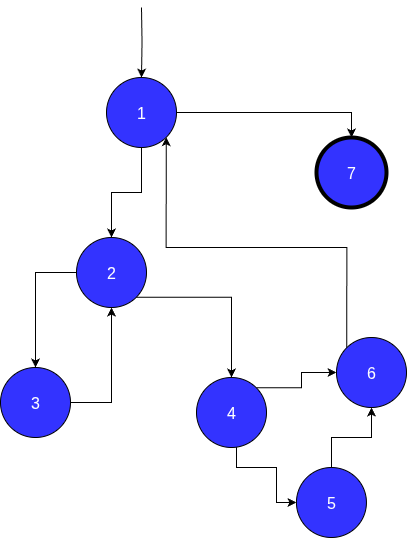
\includegraphics[width=0.5\textwidth]{hw2/q1_graph.png}

% \textbf{REMOVE THE FOLLOWING BEFORE RELEASE.}
% \VerbatimInput{hw2/q1_new_code.c}
% \textbf{REMOVE THE ABOVE BEFORE RELEASE.}

\begin{parts}
\part[4] List the Testing Requirements for Node Coverage.
\answerspace{10}
\answer{
    TR = \{1, 2, 3, 4, 5, 6, 7\}
}
\part[5] List the Testing Requirements for Edge Coverage.
\answerspace{10}
\answer{
		TR = \{ [1,2], [1,7], [2, 3], [2, 4], [3, 2], [4, 5], [4, 6], [5, 6], [6, 1]\}
}
% \part[15] List all Simple Paths
% \answerspace{10}
% \answer{
% 	[1, 2, 8],
% 	[1, 3, 8],
% 	[1, 3, 4, 5, 7],
% 	[1, 3, 4, 6, 7],
% 	[2, 8],
% 	[3, 8],
% 	[3, 4, 5, 7, 3],
% 	[3, 4, 6, 7, 3],
% 	[4, 5, 7, 3, 8],
% 	[4, 5, 7, 3, 4],
% 	[4, 6, 7, 3, 8],
% 	[4, 6, 7, 3, 4],
% 	[5, 7, 3, 8],
% 	[5, 7, 3, 4, 5],
% 	[5, 7, 3, 4, 6],
% 	[6, 7, 3, 8],
% 	[6, 7, 3, 4, 5],
% 	[6, 7, 3, 4, 6],
% 	[7, 3, 8],
% 	[7, 3, 4, 5, 7],
% 	[7, 3, 4, 6, 7]
% }
\part[15] How many prime paths exist in this graph?

\answerspace{10}
\answer{
	There are in total 15 prime paths in the given graph.
}
\part[8] How many edge-pairs exist in this graph?
\answerspace{10}
\answer{
    There are in total 13 edge-pairs in the given graph.
	(We accept 12 also as the answer here.)
}
\end{parts}

\newpage

\question Given the following graph, where the starting and terminal nodes are labeled 1 and 6, respectively:

Unless otherwise noted, assume $def(l) = \emptyset$ and $use(l) = \emptyset$.

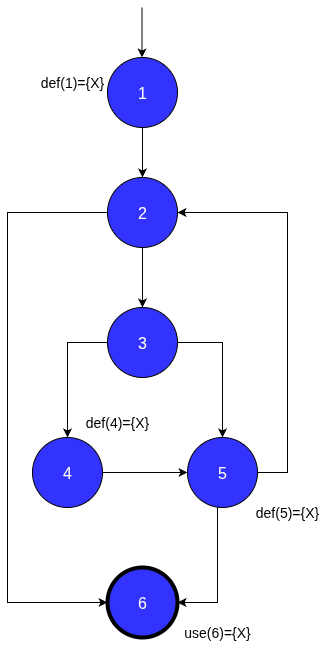
\includegraphics[width=0.5\textwidth]{hw2/graph2.png}

And the following test paths: \\
T1 = [1, 2, 3, 4, 5, 6] \\
T2 = [1, 2, 3, 5, 6] \\
T3 = [1, 2, 3, 5, 2, 6] \\
T4 = [1, 2, 6] \\
\\

\begin{parts}
\part[10] List all the DU-paths with respect to $X$. (Note: Include \textbf{all} DU-paths, even those that are subpaths of other DU-paths).

Please use the format:

\begin{center}
	du (node \#, node \#, variable name): [node \#, node \#, ...]
\end{center}

\answerspace{10}
\answer{
    \\
		du (1, 6, $X$): [1, 2, 6] \\
		du (4, 6, $X$): [ ] \\
		du (5, 6, $X$): [5, 2, 6], [5, 6] \\
}


\part[3] Which DU paths does T1 tour directly? 
Please format your answer as 
\begin{center}
	T1 tours {[n0,n1,...], …}
\end{center}
\answerspace{10}
\answer{
    \\
    T1 tours [5, 6] \\
}

\part[3] Which DU paths does T2 tour directly? 
Please format your answer as 
\begin{center}
	T2 tours {[n0,n1,...], …}
\end{center}

\answerspace{10}
\answer{
    \\
    T2 tours [5, 6] \\
}

\part[3] Which DU paths does T3 tour directly? 
Please format your answer as 
\begin{center}
	T3 tours {[n0,n1,...], …}
\end{center}


\answerspace{10}
\answer{
    \\
    T3 tours [5, 2, 6] \\
}

\part[3] Which DU paths does T4 tour directly? 
Please format your answer as 
\begin{center}
	T4 tours {[n0,n1,...], …}
\end{center}

\answerspace{10}
\answer{
    \\
    T4 tours [1, 2, 6] \\
}





\part[5] List a minimal subset of \{T1,T2,T3,T4\} that satisfies all-defs coverage with respect to $X$ (consider direct tours only). 
\answerspace{10}
\answer{
		% def2, def1, def5
            \{t1, t4\}
		Answer can also be {t2 , t4}
}

\part[5] List a minimal subset of \{T1,T2,T3,T4\} that satisfies all-uses coverage with respect to $X$ (consider direct tours only).
\answerspace{10}
\answer{
    \{t2,t4\} 
	Answer can also be {t1, t4} and {t3, t4}
}

\part[7] List a minimal subset of \{T1,T2,T3,T4\} that satisfies all-du-paths coverage with respect to $X$ (consider direct tours only).
\answerspace{10}
\answer{
		% d1 -> u8: t2
		% d1 -> u7: t4
		% d2 -> u8: t1
		% d5 -> u7: t3
		% d5 -> u8: t3
		% \{t1, t2, t3, t4\}

		% OR 

		\{t1, t3, t4\}
            or 
            \{t2, t3, t4\}
}
\end{parts}

\question Answer the following questions regarding subsumption:
\begin{parts}
\part[10] Does Node Coverage subsume Edge Coverage? Justify your answer.
\answerspace{10}
\answer{
    No, node coverage doesn't subsume edge coverage as covering all nodes does not guarantee covering all edges.
}
\part[10] Does Edge Coverage subsume Edge Pair Coverage? Justify your answer.
\answerspace{10}
\answer{
    No. Edge Coverage ensures each single edge is covered, not the coverage of all pairs of consecutive edges.
}
% \part[11] Does Edge Pair Coverage subsume Prime Path Coverage? Justify your answer.
% \answerspace{10}
% \answer{
%     No. Prime path coverage requires all maximal simple paths. Due to this, there cannot be more than 2 edges. 
% }

\part[11] Does Prime Path Coverage subsume All-DU-path Coverage? Justify your answer.
\answerspace{10}
\answer{
	Yes. The TR for All-DU-path coverage includes DU-paths only, which, by definition, must be simple paths. Since simple paths are prime paths and PPC requires coverage of all prime paths, prime path coverage subsumes all-DU-path coverage.
}
\end{parts}


\question Consider the following program and answer the questions below:
\VerbatimInput{hw2/q4_1_code.c}
Execution order: \\
Step 1. \textbf{T1:} L(A) \\
Step 2. \textbf{T2:} W(x) \\
Step 3. \textbf{T1:} W(x) \\
Step 4. \textbf{T1:} U(A) \\
\\
\textbf{Answer format:} When writing candidate locksets or held locks, always use curly braces 
(\texttt{\{\}}). 
For example: \texttt{\{\}} (empty set), \texttt{\{A\}}, \texttt{\{A, B\}}. Do not write \texttt{None}, \texttt{empty} or leave the text field empty.\\

\begin{parts}

\part[2] Locks held at step 2: (Use the \textbf{answer format} specified above)
\answerspace{10}
\answer{
	\{\}
}
\part[2] Candidate lockset after step 2: (Use the \textbf{answer format} specified above)
\answerspace{10}
\answer{
	\{\}
}
\part[2] Locks held at step 3: (Use the \textbf{answer format} specified above)
\answerspace{10}
\answer{
	\{A\}
}
\part[2] Candidate lockset after step 3: (Use the \textbf{answer format} specified above)
\answerspace{10}
\answer{
	\{\}
}
\part[2] Does the lockset race algorithm report a potential data race on this execution?
\answerspace{10}
\answer{
	Yes. The intersection of candidate set and held lock set is empty after step 3, so the lockset algorithm flags a potential race.
}
\part[2] Is this an actual race?
\answerspace{10}
\answer{
	Yes. T2 writes to \texttt{x} without holding \texttt{A} while T1 writes while holding \texttt{A}.
}


Consider the following program:
\VerbatimInput{hw2/q4_2_code.c}

Execution order: \\
Step 1. \textbf{Main:} \texttt{pthread\_create(Worker)} \\
Step 2. \textbf{Worker:} W(x) \\
Step 3. \textbf{Worker:} finishes \\
Step 4. \textbf{Main:} \texttt{pthread\_join} returns \\
Step 5. \textbf{Main:} R(x) \\

\textbf{Answer format:} When writing candidate locksets or held locks, always use curly braces 
(\texttt{\{\}}). 
For example: \texttt{\{\}} (empty set), \texttt{\{A\}}, \texttt{\{A, B\}}. Do not write \texttt{None}, \texttt{empty} or leave the text field empty.\\


% \pf{Add the required format. Show the points properly like the change I made above. Ask to follow the format in each question. Ask for explanations in the lock set and the race conclusion.}


\part[2] Locks held at step 2 (Use the \textbf{answer format} specified above):
\answerspace{10}
\answer{
	\{\}
}
\part[2] Candidate lockset after step 2 (Use the \textbf{answer format} specified above):
\answerspace{10}
\answer{
	\{\}
}
\part[2] Locks held at step 5 (Use the \textbf{answer format} specified above):
\answerspace{10}
\answer{
	\{\}
}
\part[2] Candidate lockset after step 5 (Use the \textbf{answer format} specified above):
\answerspace{10}
\answer{
	\{\}
}
\part[2] Does the lockset race algorithm report a potential data race on this execution?
\answerspace{10}
\answer{
	Yes. The intersection of candidate set and held lock set is empty after step 5, so the lockset algorithm flags a potential race.
}
\part[2] Is this an actual race?
\answerspace{10}
\answer{
	No. The join ensures the worker finishes before the main thread reads \texttt{x}, so the accesses are ordered.
}
\end{parts}


\if 0 %%%%%%%%%%%%%%%%%%%%%%%%%%%%%%%%%%%%%%%%%
	\question[10]
	\answerspace{30}
	\answer{}

	\question
	\begin{parts}
		\part[6]
		\answerspace{20}
		\answer{}

		\part[2]
		\answerspace{10}
		\answer{}

	\end{parts}
\fi %%%%%%%%%%%%%%%%%%%%%%%%%%%%%%%%%%%%%%%%%

	\newpage
	\begin{center}
		[EMPTY PAGE]
	\end{center}

\end{questions}

\end{document}
